\documentclass[]{article}
\usepackage{lmodern}
\usepackage{amssymb,amsmath}
\usepackage{ifxetex,ifluatex}
\usepackage{fixltx2e} % provides \textsubscript
\ifnum 0\ifxetex 1\fi\ifluatex 1\fi=0 % if pdftex
  \usepackage[T1]{fontenc}
  \usepackage[utf8]{inputenc}
\else % if luatex or xelatex
  \ifxetex
    \usepackage{mathspec}
  \else
    \usepackage{fontspec}
  \fi
  \defaultfontfeatures{Ligatures=TeX,Scale=MatchLowercase}
\fi
% use upquote if available, for straight quotes in verbatim environments
\IfFileExists{upquote.sty}{\usepackage{upquote}}{}
% use microtype if available
\IfFileExists{microtype.sty}{%
\usepackage[]{microtype}
\UseMicrotypeSet[protrusion]{basicmath} % disable protrusion for tt fonts
}{}
\PassOptionsToPackage{hyphens}{url} % url is loaded by hyperref
\usepackage[unicode=true]{hyperref}
\hypersetup{
            pdftitle={Regression Models Course Project},
            pdfborder={0 0 0},
            breaklinks=true}
\urlstyle{same}  % don't use monospace font for urls
\usepackage[margin=1in]{geometry}
\usepackage{color}
\usepackage{fancyvrb}
\newcommand{\VerbBar}{|}
\newcommand{\VERB}{\Verb[commandchars=\\\{\}]}
\DefineVerbatimEnvironment{Highlighting}{Verbatim}{commandchars=\\\{\}}
% Add ',fontsize=\small' for more characters per line
\usepackage{framed}
\definecolor{shadecolor}{RGB}{248,248,248}
\newenvironment{Shaded}{\begin{snugshade}}{\end{snugshade}}
\newcommand{\KeywordTok}[1]{\textcolor[rgb]{0.13,0.29,0.53}{\textbf{#1}}}
\newcommand{\DataTypeTok}[1]{\textcolor[rgb]{0.13,0.29,0.53}{#1}}
\newcommand{\DecValTok}[1]{\textcolor[rgb]{0.00,0.00,0.81}{#1}}
\newcommand{\BaseNTok}[1]{\textcolor[rgb]{0.00,0.00,0.81}{#1}}
\newcommand{\FloatTok}[1]{\textcolor[rgb]{0.00,0.00,0.81}{#1}}
\newcommand{\ConstantTok}[1]{\textcolor[rgb]{0.00,0.00,0.00}{#1}}
\newcommand{\CharTok}[1]{\textcolor[rgb]{0.31,0.60,0.02}{#1}}
\newcommand{\SpecialCharTok}[1]{\textcolor[rgb]{0.00,0.00,0.00}{#1}}
\newcommand{\StringTok}[1]{\textcolor[rgb]{0.31,0.60,0.02}{#1}}
\newcommand{\VerbatimStringTok}[1]{\textcolor[rgb]{0.31,0.60,0.02}{#1}}
\newcommand{\SpecialStringTok}[1]{\textcolor[rgb]{0.31,0.60,0.02}{#1}}
\newcommand{\ImportTok}[1]{#1}
\newcommand{\CommentTok}[1]{\textcolor[rgb]{0.56,0.35,0.01}{\textit{#1}}}
\newcommand{\DocumentationTok}[1]{\textcolor[rgb]{0.56,0.35,0.01}{\textbf{\textit{#1}}}}
\newcommand{\AnnotationTok}[1]{\textcolor[rgb]{0.56,0.35,0.01}{\textbf{\textit{#1}}}}
\newcommand{\CommentVarTok}[1]{\textcolor[rgb]{0.56,0.35,0.01}{\textbf{\textit{#1}}}}
\newcommand{\OtherTok}[1]{\textcolor[rgb]{0.56,0.35,0.01}{#1}}
\newcommand{\FunctionTok}[1]{\textcolor[rgb]{0.00,0.00,0.00}{#1}}
\newcommand{\VariableTok}[1]{\textcolor[rgb]{0.00,0.00,0.00}{#1}}
\newcommand{\ControlFlowTok}[1]{\textcolor[rgb]{0.13,0.29,0.53}{\textbf{#1}}}
\newcommand{\OperatorTok}[1]{\textcolor[rgb]{0.81,0.36,0.00}{\textbf{#1}}}
\newcommand{\BuiltInTok}[1]{#1}
\newcommand{\ExtensionTok}[1]{#1}
\newcommand{\PreprocessorTok}[1]{\textcolor[rgb]{0.56,0.35,0.01}{\textit{#1}}}
\newcommand{\AttributeTok}[1]{\textcolor[rgb]{0.77,0.63,0.00}{#1}}
\newcommand{\RegionMarkerTok}[1]{#1}
\newcommand{\InformationTok}[1]{\textcolor[rgb]{0.56,0.35,0.01}{\textbf{\textit{#1}}}}
\newcommand{\WarningTok}[1]{\textcolor[rgb]{0.56,0.35,0.01}{\textbf{\textit{#1}}}}
\newcommand{\AlertTok}[1]{\textcolor[rgb]{0.94,0.16,0.16}{#1}}
\newcommand{\ErrorTok}[1]{\textcolor[rgb]{0.64,0.00,0.00}{\textbf{#1}}}
\newcommand{\NormalTok}[1]{#1}
\usepackage{longtable,booktabs}
% Fix footnotes in tables (requires footnote package)
\IfFileExists{footnote.sty}{\usepackage{footnote}\makesavenoteenv{long table}}{}
\usepackage{graphicx,grffile}
\makeatletter
\def\maxwidth{\ifdim\Gin@nat@width>\linewidth\linewidth\else\Gin@nat@width\fi}
\def\maxheight{\ifdim\Gin@nat@height>\textheight\textheight\else\Gin@nat@height\fi}
\makeatother
% Scale images if necessary, so that they will not overflow the page
% margins by default, and it is still possible to overwrite the defaults
% using explicit options in \includegraphics[width, height, ...]{}
\setkeys{Gin}{width=\maxwidth,height=\maxheight,keepaspectratio}
\IfFileExists{parskip.sty}{%
\usepackage{parskip}
}{% else
\setlength{\parindent}{0pt}
\setlength{\parskip}{6pt plus 2pt minus 1pt}
}
\setlength{\emergencystretch}{3em}  % prevent overfull lines
\providecommand{\tightlist}{%
  \setlength{\itemsep}{0pt}\setlength{\parskip}{0pt}}
\setcounter{secnumdepth}{0}
% Redefines (sub)paragraphs to behave more like sections
\ifx\paragraph\undefined\else
\let\oldparagraph\paragraph
\renewcommand{\paragraph}[1]{\oldparagraph{#1}\mbox{}}
\fi
\ifx\subparagraph\undefined\else
\let\oldsubparagraph\subparagraph
\renewcommand{\subparagraph}[1]{\oldsubparagraph{#1}\mbox{}}
\fi

% set default figure placement to htbp
\makeatletter
\def\fps@figure{htbp}
\makeatother


\title{Regression Models Course Project}
\author{}
\date{\vspace{-2.5em}}

\begin{document}
\maketitle

Supposing I work for \emph{Motor Trend}, a magazine about the automobile
industry. Looking at a data set of a collection of cars, they are
interested in exploring the relationship between a set of variables and
miles per gallon (MPG) (outcome). They are particularly interested in
the following two questions:

\begin{itemize}
\tightlist
\item
  \textbf{``Is an automatic or manual transmission better for MPG''}
\item
  \textbf{``Quantify the MPG difference between automatic and manual
  transmissions''}
\end{itemize}

\subsection{\texorpdfstring{\textbf{1. Loading
Data}}{1. Loading Data}}\label{loading-data}

We load the dataset

\begin{Shaded}
\begin{Highlighting}[]
\KeywordTok{data}\NormalTok{(mtcars)}
\KeywordTok{head}\NormalTok{(mtcars)}
\end{Highlighting}
\end{Shaded}

\begin{verbatim}
##                    mpg cyl disp  hp drat    wt  qsec vs am gear carb
## Mazda RX4         21.0   6  160 110 3.90 2.620 16.46  0  1    4    4
## Mazda RX4 Wag     21.0   6  160 110 3.90 2.875 17.02  0  1    4    4
## Datsun 710        22.8   4  108  93 3.85 2.320 18.61  1  1    4    1
## Hornet 4 Drive    21.4   6  258 110 3.08 3.215 19.44  1  0    3    1
## Hornet Sportabout 18.7   8  360 175 3.15 3.440 17.02  0  0    3    2
## Valiant           18.1   6  225 105 2.76 3.460 20.22  1  0    3    1
\end{verbatim}

Motor Trend Car Road Tests

\emph{Description}

The data was extracted from the 1974 Motor Trend US magazine, and
comprises fuel consumption and 10 aspects of automobile design and
performance for 32 automobiles (1973-74 models).

\emph{Format}

A data frame with 32 observations on 11 (numeric) variables.

\begin{longtable}[]{@{}lll@{}}
\toprule
{[}, 1{]} & mpg & Miles/(US) gallon\tabularnewline
{[}, 2{]} & cyl & Number of cylinders\tabularnewline
{[}, 3{]} & disp & Displacement (cu.in.)\tabularnewline
{[}, 4{]} & hp & Gross horsepower\tabularnewline
{[}, 5{]} & drat & Rear axle ratio\tabularnewline
{[}, 6{]} & wt & Weight (1000 lbs)\tabularnewline
{[}, 7{]} & qsec & 1/4 mile time\tabularnewline
{[}, 8{]} & vs & Engine (0 = V-shaped, 1 = straight)\tabularnewline
{[}, 9{]} & am & Transmission (0 = automatic, 1 = manual)\tabularnewline
{[},10{]} & gear & Number of forward gears\tabularnewline
{[},11{]} & carb & Number of carburetors\tabularnewline
\bottomrule
\end{longtable}

\begin{verbatim}
## Loading required package: carData
\end{verbatim}

\begin{verbatim}
## Loading required package: ggplot2
\end{verbatim}

\begin{verbatim}
## Registered S3 method overwritten by 'GGally':
##   method from   
##   +.gg   ggplot2
\end{verbatim}

For convenience we can convert the variable ``am'' to a factor and add a
more clear classification ``Automatic'' \& ``Manual''. and we can
perform a friefly analysis of both variables

\begin{Shaded}
\begin{Highlighting}[]
\NormalTok{mtcars}\OperatorTok{$}\NormalTok{am =}\StringTok{ }\KeywordTok{as.factor}\NormalTok{(mtcars}\OperatorTok{$}\NormalTok{am)}
\KeywordTok{levels}\NormalTok{(mtcars}\OperatorTok{$}\NormalTok{am) =}\StringTok{ }\KeywordTok{c}\NormalTok{(}\StringTok{"Automatic"}\NormalTok{, }\StringTok{"Manual"}\NormalTok{)}
\KeywordTok{summary}\NormalTok{(mtcars}\OperatorTok{$}\NormalTok{mpg); }\KeywordTok{summary}\NormalTok{(mtcars}\OperatorTok{$}\NormalTok{am)}
\end{Highlighting}
\end{Shaded}

\begin{verbatim}
##    Min. 1st Qu.  Median    Mean 3rd Qu.    Max. 
##   10.40   15.43   19.20   20.09   22.80   33.90
\end{verbatim}

\begin{verbatim}
## Automatic    Manual 
##        19        13
\end{verbatim}

\section{\texorpdfstring{\textbf{2.EDA}}{2.EDA}}\label{eda}

\begin{Shaded}
\begin{Highlighting}[]
\KeywordTok{scatterplotMatrix}\NormalTok{(}\OperatorTok{~}\NormalTok{mpg}\OperatorTok{+}\NormalTok{disp}\OperatorTok{+}\NormalTok{drat}\OperatorTok{+}\NormalTok{wt}\OperatorTok{+}\NormalTok{hp}\OperatorTok{|}\NormalTok{am, }\DataTypeTok{data=}\NormalTok{mtcars, }\DataTypeTok{col =} \KeywordTok{c}\NormalTok{(}\StringTok{"skyblue4"}\NormalTok{, }\StringTok{"indianred4"}\NormalTok{), }\DataTypeTok{main=}\StringTok{"Type of Transmission"}\NormalTok{, }\DataTypeTok{cex.labels=} \DecValTok{1}\NormalTok{,}\DataTypeTok{cex.main=}\DecValTok{2}\NormalTok{, }\DataTypeTok{cex=}\FloatTok{1.5}\NormalTok{)}
\end{Highlighting}
\end{Shaded}

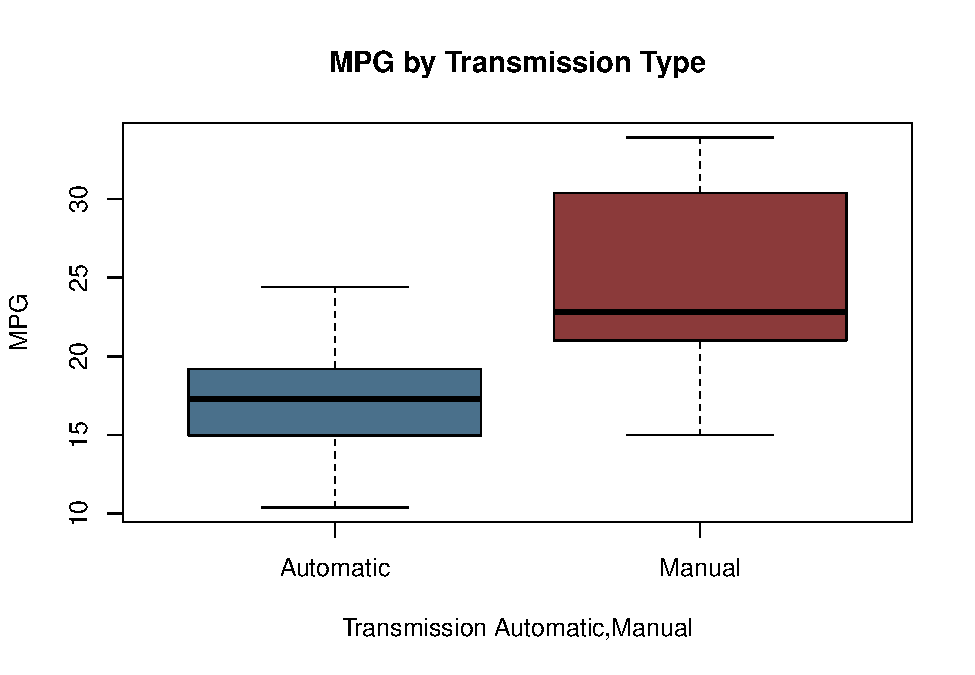
\includegraphics{Final_files/figure-latex/unnamed-chunk-5-1.pdf}

\begin{Shaded}
\begin{Highlighting}[]
\KeywordTok{boxplot}\NormalTok{(mpg}\OperatorTok{~}\NormalTok{am,}\DataTypeTok{data =}\NormalTok{ mtcars,}\DataTypeTok{xlab =} \StringTok{"Transmission Automatic,Manual"}\NormalTok{, }\DataTypeTok{ylab =} \StringTok{"MPG"}\NormalTok{, }\DataTypeTok{main=}\StringTok{"MPG by Transmission Type"}\NormalTok{, }\DataTypeTok{col=}\KeywordTok{c}\NormalTok{(}\StringTok{"skyblue4"}\NormalTok{, }\StringTok{"indianred4"}\NormalTok{))}
\end{Highlighting}
\end{Shaded}

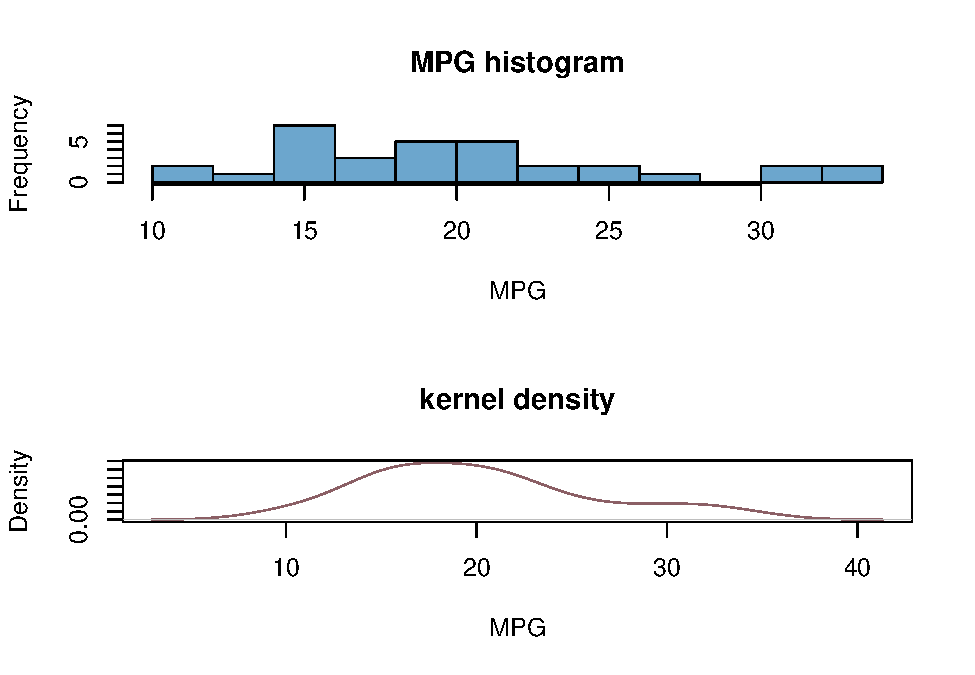
\includegraphics{Final_files/figure-latex/unnamed-chunk-6-1.pdf}
\#\textbf{3. t-test}

\begin{Shaded}
\begin{Highlighting}[]
\KeywordTok{hist}\NormalTok{(mtcars}\OperatorTok{$}\NormalTok{mpg, }\DataTypeTok{breaks=}\DecValTok{10}\NormalTok{, }\DataTypeTok{xlab=}\StringTok{"MPG"}\NormalTok{, }\DataTypeTok{main=}\StringTok{"MPG histogram"}\NormalTok{, }\DataTypeTok{col =} \StringTok{"skyblue3"}\NormalTok{)}
\end{Highlighting}
\end{Shaded}

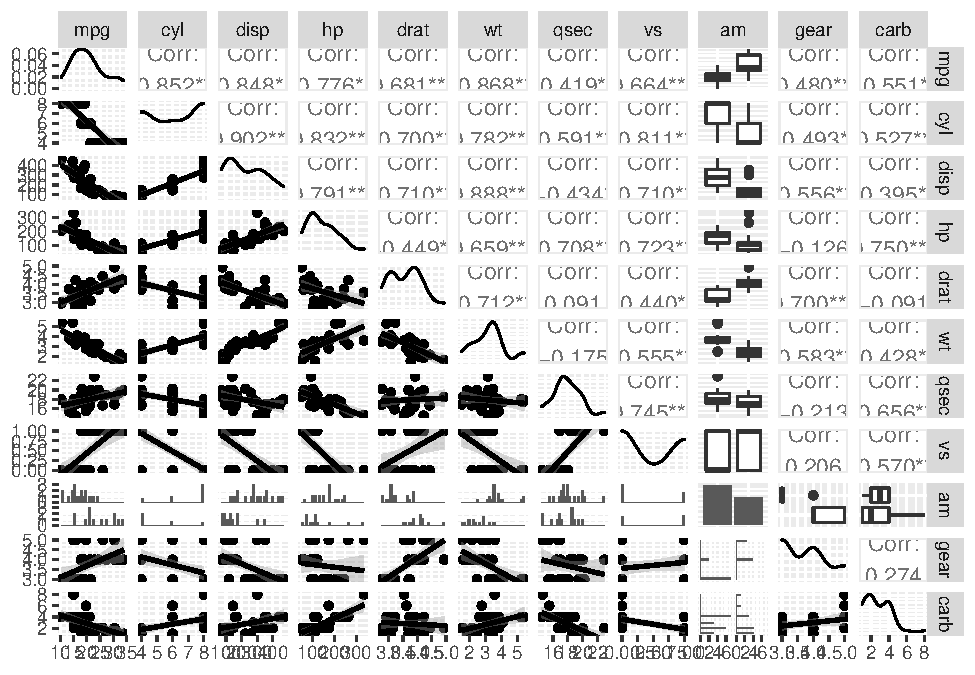
\includegraphics{Final_files/figure-latex/unnamed-chunk-7-1.pdf}

\begin{Shaded}
\begin{Highlighting}[]
\KeywordTok{plot}\NormalTok{(}\KeywordTok{density}\NormalTok{(mtcars}\OperatorTok{$}\NormalTok{mpg), }\DataTypeTok{main=}\StringTok{"kernel density"}\NormalTok{, }\DataTypeTok{xlab=}\StringTok{"MPG"}\NormalTok{, }\DataTypeTok{col=}\StringTok{"lightpink4"}\NormalTok{ )}
\end{Highlighting}
\end{Shaded}

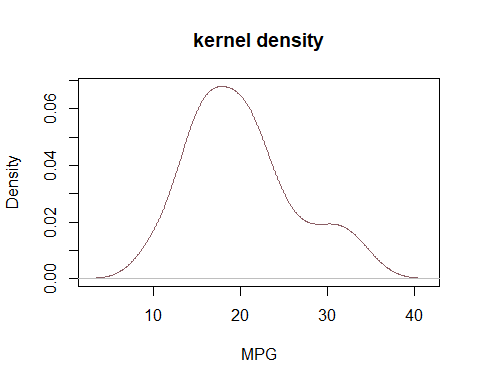
\includegraphics{Final_files/figure-latex/unnamed-chunk-8-1.pdf}

\begin{Shaded}
\begin{Highlighting}[]
\KeywordTok{library}\NormalTok{(GGally)}
\KeywordTok{library}\NormalTok{(ggplot2)    }

\NormalTok{gp =}\StringTok{ }\KeywordTok{ggpairs}\NormalTok{(mtcars, }\DataTypeTok{lower =} \KeywordTok{list}\NormalTok{(}\DataTypeTok{continuous =} \StringTok{"smooth"}\NormalTok{))}
\NormalTok{gp}
\end{Highlighting}
\end{Shaded}

\begin{verbatim}
## `stat_bin()` using `bins = 30`. Pick better value with `binwidth`.
## `stat_bin()` using `bins = 30`. Pick better value with `binwidth`.
## `stat_bin()` using `bins = 30`. Pick better value with `binwidth`.
## `stat_bin()` using `bins = 30`. Pick better value with `binwidth`.
## `stat_bin()` using `bins = 30`. Pick better value with `binwidth`.
## `stat_bin()` using `bins = 30`. Pick better value with `binwidth`.
## `stat_bin()` using `bins = 30`. Pick better value with `binwidth`.
## `stat_bin()` using `bins = 30`. Pick better value with `binwidth`.
## `stat_bin()` using `bins = 30`. Pick better value with `binwidth`.
## `stat_bin()` using `bins = 30`. Pick better value with `binwidth`.
\end{verbatim}

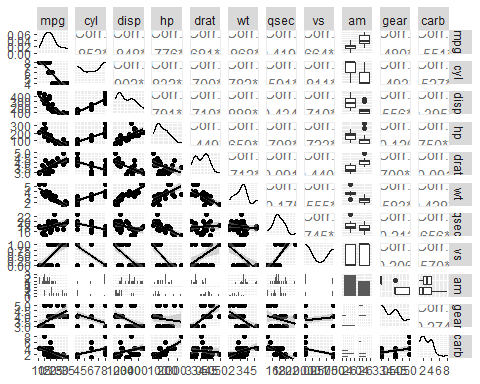
\includegraphics{Final_files/figure-latex/unnamed-chunk-9-1.pdf}
Interpretation : In this plot, we see many multi-collinearity, and it
suggests that we should NOT use all the variables as predictor otherwise
it will be overfitting.

\section{\texorpdfstring{\textbf{4.Quantify the MPG difference between
automatic and manual
transmissions}}{4.Quantify the MPG difference between automatic and manual transmissions}}\label{quantify-the-mpg-difference-between-automatic-and-manual-transmissions}

Consider all the other varaibles as possible predictor and MPG as
outcome. Use R step function to find out the best fit model

First, Glimpse at all relationship between each variable

\textbf{Finding best model}

\begin{Shaded}
\begin{Highlighting}[]
\NormalTok{best_model<-}\KeywordTok{step}\NormalTok{(}\KeywordTok{lm}\NormalTok{(mpg }\OperatorTok{~}\StringTok{ }\NormalTok{.,}\DataTypeTok{data =}\NormalTok{ mtcars), }\DataTypeTok{trace=}\DecValTok{0}\NormalTok{)}
\KeywordTok{summary}\NormalTok{(best_model)}
\end{Highlighting}
\end{Shaded}

\begin{verbatim}
## 
## Call:
## lm(formula = mpg ~ wt + qsec + am, data = mtcars)
## 
## Residuals:
##     Min      1Q  Median      3Q     Max 
## -3.4811 -1.5555 -0.7257  1.4110  4.6610 
## 
## Coefficients:
##             Estimate Std. Error t value Pr(>|t|)    
## (Intercept)   9.6178     6.9596   1.382 0.177915    
## wt           -3.9165     0.7112  -5.507 6.95e-06 ***
## qsec          1.2259     0.2887   4.247 0.000216 ***
## amManual      2.9358     1.4109   2.081 0.046716 *  
## ---
## Signif. codes:  0 '***' 0.001 '**' 0.01 '*' 0.05 '.' 0.1 ' ' 1
## 
## Residual standard error: 2.459 on 28 degrees of freedom
## Multiple R-squared:  0.8497, Adjusted R-squared:  0.8336 
## F-statistic: 52.75 on 3 and 28 DF,  p-value: 1.21e-11
\end{verbatim}

\begin{Shaded}
\begin{Highlighting}[]
\CommentTok{#par(mfrow=c(2,2))}
\KeywordTok{plot}\NormalTok{(best_model)}
\end{Highlighting}
\end{Shaded}

\includegraphics{Final_files/figure-latex/unnamed-chunk-11-1.pdf}
\includegraphics{Final_files/figure-latex/unnamed-chunk-11-2.pdf}
\includegraphics{Final_files/figure-latex/unnamed-chunk-11-3.pdf}
\includegraphics{Final_files/figure-latex/unnamed-chunk-11-4.pdf} We can
conclude that the best model are with wt/qsec/am as predictor and the
R-square is 84.97\%, which is good fitting to mpg outcome.The mpg of
manual cars is 2.9358 mpg better than that of automatic cars.

\end{document}
